\documentclass[center]{beamer}

\usetheme[compress]{Singapore}

% Do not show subsection markers in the headline 
\setbeamertemplate{Singapore subsection in head/foot}{use=false}
\setbeamercovered{transparent}
% Remove navigation symbols in the bottom of the slides
\beamertemplatenavigationsymbolsempty 
% \newcommand\independent{\protect\mathpalette{\protect\independenT}{\perp}}
% \def\independenT#1#2{\mathrel{\rlap{$#1#2$}\mkern2mu{#1#2}}}


\usepackage{marvosym}
\usepackage{graphicx}
\usepackage[backend      = biber,     
            isbn         = false,     
            doi          = false,     
            url          = false,     
            eprint       = false,    
            style        = alphabetic,
            maxcitenames = 1,         
            maxbibnames  = 3,         
            uniquelist   = false]{biblatex}
\addbibresource{/home/bach/Documents/papers/BIB/references.bib}
\usepackage{amsmath}
\usepackage{amsthm}
\usepackage{amsfonts}
\usepackage{amssymb}
\usepackage{mathtools}
\mathtoolsset{showonlyrefs=true}
\usepackage{booktabs}

\let\oldcite\cite
\renewcommand{\cite}[1]{\textcolor{gray}{\oldcite{#1}}}

\newcommand{\ex}[1]{{\usebeamercolor[fg]{block title example} #1}}


% Configure title, authors and contact 
\title[Retention order prediction]{%
    Liquid-Chromatography Retention Order Prediction for Metabolite Identification}
    
\author[\Letter: eric.bach@aalto.fi]{ % address for correspondence 
    Eric Bach\,$^{\text{1,\Letter}}$, % 
    Sandor Szedmak\,$^{\text{1}}$,    %
    C\'eline Brouard\,$^{\text{1}}$,  %
    Sebastian B\"ocker\,$^{\text{2}}$ %
    and Juho Rousu\,$^{\text{1}}$}
    
\institute[]{%
    $^{\text{1}}$Helsinki institute for Information Technology (HIIT), Department of Computer Science, Aalto University, Espoo, Finland\\
    $^{\text{2}}$Chair for Bioinformatics, Friedrich-Schiller-University, Jena, Germany.}
  \date{ECCB conference in Athens: September 11, 2018}

% Configure beamer footline
\setbeamertemplate{footline}{%
    \leavevmode%
    \hbox{%
        \hskip3pt
        \begin{beamercolorbox}[wd=.69\paperwidth,ht=2.25ex,dp=1ex,left]{title in head/foot}%
            \usebeamerfont{title in head/foot}\inserttitle
        \end{beamercolorbox}
        \begin{beamercolorbox}[wd=.15\paperwidth,ht=2.25ex,dp=1ex,center]{author in head/foot}%
            \usebeamerfont{author in head/foot}\insertshortauthor
        \end{beamercolorbox}
        \begin{beamercolorbox}[wd=.15\paperwidth,ht=2.25ex,dp=1ex,right]{framenumber in head/foot}%
            \insertframenumber{} / \inserttotalframenumber\hspace{7pt}
        \end{beamercolorbox}
  }%
  \vskip0pt%
}

% \setbeamertemplate{headline}
% {
%     \leavevmode
%     \begin{beamercolorbox}{section in head/foot}
%     \vskip2pt\insertsectionnavigationhorizontal{\textwidth}{}{}\vskip2pt
%     \end{beamercolorbox}
% }

% Load notations
% Notations
\newcommand{\VEC}[1]{\mathbf{#1}}
\newcommand{\mol}{m}
\newcommand{\sys}{s}
\newcommand{\ms}{x}
\newcommand{\molspace}{\mathcal{M}}
\newcommand{\sysspace}{\mathcal{S}}
\newcommand{\msspace}{\mathcal{X}}
\newcommand{\rettimespace}{\mathbb{R}_{+}}
\newcommand{\Kpw}{\mathbf{Q}} % pairwise kernel K: p x p
\newcommand{\Kmol}{\mathbf{K}_{m}} % molecule kernel K_phi: l x l
\newcommand{\Ksys}{\mathbf{K}_{\Psi}} % system kernel K_phi: l x l
\newcommand{\kmol}{k_m} % kernel between molecules
\newcommand{\kms}{k_x} % kernel between tandem mass spectra
\newcommand{\Fmol}{\mathcal{F}_m} % feature space for molecules
\newcommand{\Fms}{\mathcal{F}_x} % feature space for tandem mass spectra
\newcommand{\Pref}{\mathcal{P}}
\newcommand{\RTimes}{\mathcal{T}}
\newcommand{\sgn}{\mathrm{sign}}
\DeclareMathOperator*{\argmax}{argmax}


\begin{document}

% Title frame
\frame[noframenumbering]{ \thispagestyle{empty} 
    \titlepage 
    % Insert logos
    
\includegraphics[scale=0.25]{images/aalto_logo.pdf}
    \hfill
    
\includegraphics[scale=0.25]{images/hiit_logo.pdf}
}

% Motivation frame
% \frame{ %\thispagestyle{empty} 
%     \frametitle{Motivation / Background}
% }

% Table of content


\section[LC \& Proposed method]{Liquid chromatography}
\frame{
    \frametitle{Predicting retention orders from different systems} 
}

\frame{
    \frametitle{Integrating predicted retention orders and MSMS scores} 
}
  

\section[Retention order prediction]{Ranking Support Vector Machine for order prediction}
\frame{
    \frametitle{Retention order pairs for preference learning}
    
\begin{block}{Notation}
\begin{itemize}
    \item Molecule $\mol_i$ from the molecular space $\molspace$
    \item $t_i\in\rettimespace$ its retention time
    \item $\sys_i\in\sysspace$ chromatographic system it has been measured with
\end{itemize}
\end{block}
\begin{block}{Pairwise molecule preference}
\begin{itemize}
    \item $\mol_i$ is preferred over $\mol_j$ when it \emph{elutes before} $\mol_j$, i.e. $t_i<t_j$
    \item Set of pairwise preferences of given LC-system $\sys$ is defined as:
\vspace{-0.15cm}
\begin{equation}
    \Pref(s)=\{(i,j)\,|\,\sys_i=\sys_j=\sys,t_i<t_j\}
\end{equation}
    \item Set of pairwise preferences from \emph{multiple} LC-systems:
\vspace{-0.15cm}
\begin{equation}
    \Pref=\bigcup_{\sys \in S} \Pref(\sys)
\end{equation}    
\end{itemize}
\end{block}
}

\frame{
    \frametitle{Preference learning: Ranking Support Vector Machine}
    
    We want to learn a pairwise retention order prediction function:
\vspace{-0.15cm} 
\begin{align}
    f(\mol_i = 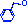
\includegraphics[scale=1.2]{images/mol_i.pdf},\mol_j = 
\includegraphics[scale=1.2]{images/mol_j.pdf} ) 
%         &= \sgn(\VEC{w}^T(\phi(\mol_j= 
\includegraphics[scale=1.2]{images/mol_j.pdf})-\phi(\mol_i= 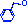
\includegraphics[scale=1.2]{images/mol_i.pdf})))\\
        &= \begin{cases}
            1  & \mol_i = 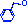
\includegraphics[scale=1.2]{images/mol_i.pdf} \text{ elutes before } \mol_j = 
\includegraphics[scale=1.2]{images/mol_j.pdf}\\
            -1 & \text{otherwise}
        \end{cases}
\end{align}

\visible<1>{
\vspace{-0.75cm}
\begin{block}{Kernelized RankSVM prediction model}
\vspace{-0.15cm}
\begin{equation}
    f(\mol_i,\mol_j) = \sgn(\VEC{w}^T(\phi(\mol_j)-\phi(\mol_i)))
\end{equation}
\vspace{-0.15cm}
\begin{itemize}
    \item $\VEC{w}$ are the RankSVM \cite{Joachims2002,Kuo2014} model parameters
    \item $\phi:\molspace\rightarrow\Fmol$ feature map associated with $\kmol$ embedding the molecular structures into a feature space.
    \item \emph{Kernel function} $\kmol:\molspace\times\molspace\rightarrow\mathcal{R}$ encodes similarity between molecular structures
\end{itemize}
\end{block}
}
}

\frame{
    \frametitle{Training the RankSVM for retention order prediction}
    
    We optimize $\VEC{w}$ considering the pairwise preferences $\Pref$ from (possibly) different chromatographic systems:
\begin{align}
    \underset{\VEC{w},\VEC{\xi}}{\min} &\quad \frac{1}{2}\VEC{w}^T\VEC{w} + C\sum_{(i,j)\in  \Pref}\xi_{ij} \\
    s.t. &\quad\VEC{w}^T(\phi(\mol_j)-\phi(\mol_i))\geq 1-\xi_{ij}, \forall(i,j)\in  \Pref\label{prob:rankSVM-primal}\\
    &\quad \xi_{ij} \geq 0, \forall(i,j)\in \Pref,
\end{align}
    with $C>0$ being the regularization parameter.

\begin{block}{Learned model}
\begin{equation}
    \VEC{w}^T\phi(\mol_i)<\VEC{w}^T\phi(\mol_j),\,\text{if}\,(i,j)\in  \Pref 
\end{equation}
\end{block}
}


% \section{Experiments: Order prediction}s
\frame{
    \frametitle{Evaluating retention order prediction}
    
\begin{block}{Dataset}
\begin{itemize}
    \item 1098 retention times of 946 unique molecular structures
    \item 5 different reversed phase LC-systems (denoted with $\hat{S}$)
\end{itemize}
\end{block}
\begin{block}{Evaluation measure and protocol}
\begin{itemize}
    \item Pairwise prediction accuracy for a target system $\sys\in\hat{S}$:
\begin{equation}
    Acc(s)\equiv\frac{|\{(i,j)\in\Pref(s)\,|\,\VEC{w}^T\phi(\mol_i)<\VEC{w}^T\phi(\mol_j)\}|}{\Pref(s)}
\end{equation}
    \item Accuracy accessed using repeated 10-fold cross-validation.
    \item no test molecular structure in the training set
\end{itemize}
\end{block}
}

\frame{ 
    \frametitle{Compare binary and counting molecular fingerprints}
%     \framesubtitle{Encoding molecular structures using MACCS dictionary molecular fingerprints.}

\begin{itemize}
    \item Pairwise prediction accuracy ($\pm 2\sigma$) for different target systems
    \item RankSVM models trained using single system $\Pref(\sys)$.
\end{itemize}

\begin{table}[!t]
\begin{tabular}{@{}lcc@{}}
    \toprule 
    Target system $\sys$ & Binary MACCS & Counting MACCS \\\midrule
    Eawag\_XBridgeC18 & $0.796 (\pm 0.015)$ & $\mathbf{0.844 (\pm 0.011)}$ \\
    FEM\_long         & $0.882 (\pm 0.016)$ & $\mathbf{0.905 (\pm 0.015)}$ \\
    RIKEN             & $0.826 (\pm 0.024)$ & $\mathbf{0.848 (\pm 0.017)}$ \\
    UFZ\_Phenomenex   & $0.790 (\pm 0.027)$ & $\mathbf{0.802 (\pm 0.017)}$ \\
    LIFE\_old         & $0.842 (\pm 0.050)$ & $\mathbf{0.862 (\pm 0.035)}$ \\
    \bottomrule
\end{tabular}
\end{table} 
}

\frame{
    \frametitle{Train model with preferences from different systems}
    \framesubtitle{Can pairwise predictor benefit from information of different systems?}

\begin{block}{Compare performance of different training sets}
\begin{itemize}
    \item Single system, target data only: $\Pref(\sys)$
    \item Multiple systems, \emph{no} target data: $\Pref\setminus\Pref(\sys)$
    \item Multiple systems, all available data: $\Pref$
    \item Varying percentage ???
\end{itemize}
\end{block}
\begin{block}{Comparison method}
\begin{itemize}
    \item Support Vector Regression (SVR) trained on retention times directly \cite{Aicheler2015}.
    \item In multiple system setting: Retention times are considered jointly.
\end{itemize}
\end{block}
}

\frame{
    \frametitle{Train model with preferences from different systems}
    \framesubtitle{Application setting: Training retention times only available from single target system.}
    
\begin{center}
    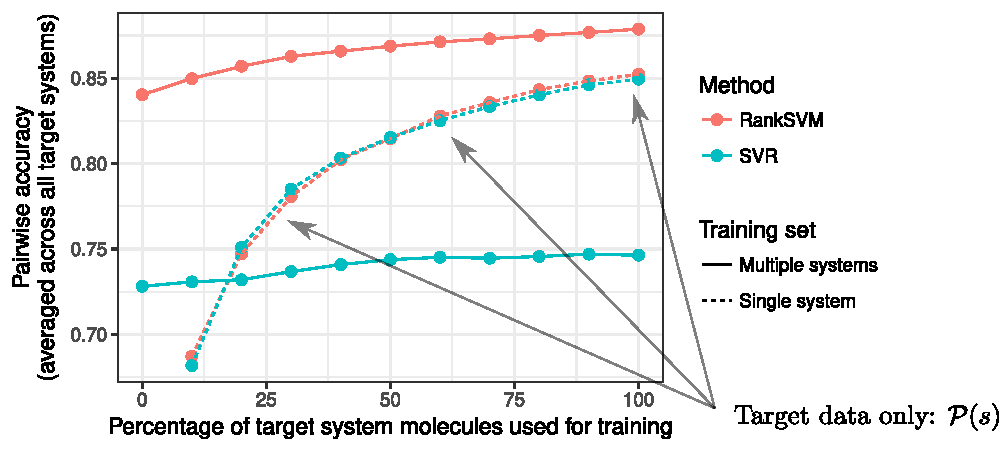
\includegraphics[width=\textwidth]{images/pwacc_2_marked_4.pdf}
\end{center}
\vspace{-0.25cm}
\begin{block}{Observations}
\begin{itemize}
    \item Increasing amount of training data improves prediction.
    \item RankSVM and SVR perform equally.
\end{itemize}
\end{block}
}

\frame{
    \frametitle{Train model with preferences from different systems}
    \framesubtitle{Application Setting: Training retention times only available \emph{from not target} system.}
    
\begin{center}
    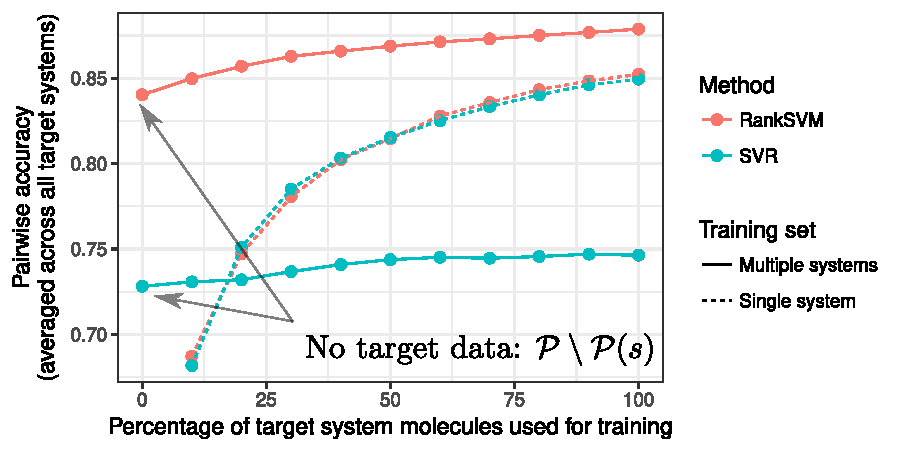
\includegraphics[width=0.9\textwidth]{images/pwacc_2_marked_2.pdf}
\end{center}
\vspace{-0.25cm}
\begin{block}{Observations}
\begin{itemize}
    \item Performance of single system \emph{without} data from the target.
    \item RankSVM outperforms SVR by considering retention \emph{orders}.
\end{itemize}
\end{block}
}

\frame{
    \frametitle{Train model with preferences from different systems}
    \framesubtitle{Application Setting: Training retention times from target \emph{and} others systems available.}
    
\begin{center}
    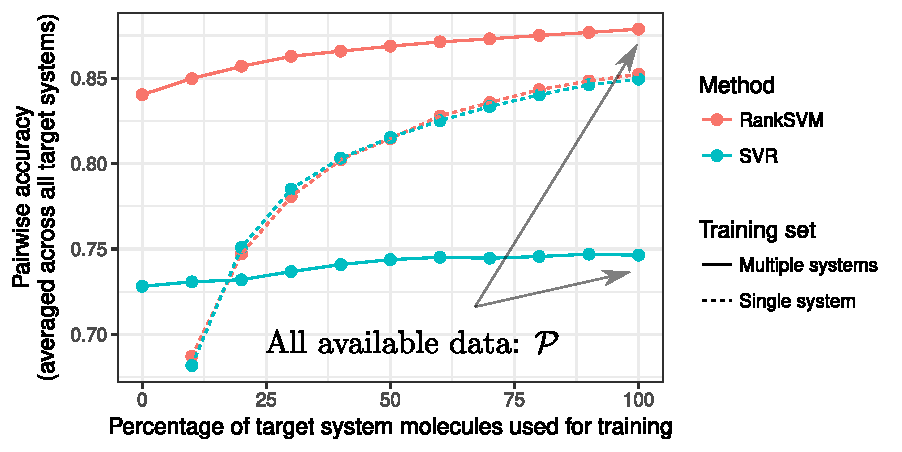
\includegraphics[width=0.9\textwidth]{images/pwacc_2_marked_3.pdf}
\end{center}
\vspace{-0.25cm}
\begin{small}
\begin{block}{Observations}
\vspace{-0.15cm}
\begin{itemize}
    \item Considering target \emph{and} non-target systems' data outperforms single system.
    \item RankSVM again outperforms SVR.
\end{itemize}
\end{block}
\end{small}
}


\section[Metabolite Identification]{Metabolite Identification}
\frame{
    \frametitle{Metabolite identification} 
    
    % we do not measure the structure. 
    % we have to infer the structure from the spectra, unlike in sequencing. 
    
\begin{small}
\begin{itemize}
    \item Small molecules ($<$ 1000 Da) involved in biological processes
    \item Identification of metabolites present in a biological sample
%     \item Widely used analysis workflow: \alert<2>{Liquid chromatography (LC)} combined with \alert<3>{tandem mass spectrometry (MS/MS)}
    \item Widely used analysis workflow: Liquid chromatography (LC) combined with tandem mass spectrometry (MS/MS)
\end{itemize}
\end{small}
\vspace{0.5cm}
% \includegraphics<2>[width=\textwidth]{images/lc_concept.pdf}
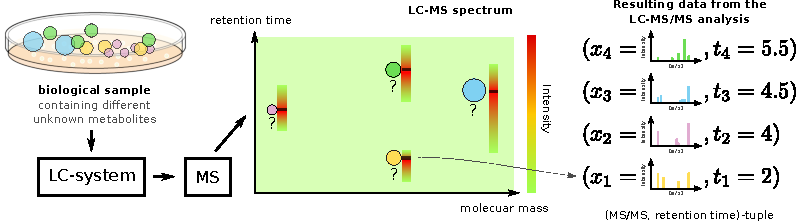
\includegraphics[width=\textwidth]{images/lcms_spectrum_complex_no_retention_order.pdf}
}

%% System LC vs Molecuar property MSMS

\frame{
    \frametitle{State-of-the-art MS/MS based metabolite identification} 

\begin{figure}[c]
    \centering
    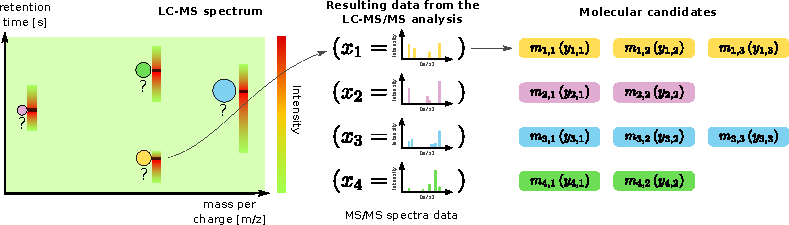
\includegraphics[width=1\textwidth]{images/lcms_spectrum_complex_small_only_iokr_with_candidates.pdf}
\end{figure}
\vspace{-0.15cm}
\begin{small}
\begin{block}{Identification workflow}
\vspace{-0.15cm}
\begin{enumerate}
    \item For each MS/MS spectra $x_i$ define a set of \emph{molecular candidate structures} $\{m_{i,1},m_{i,2},\ldots\}$.\hfill\ex{using the molecular mass}
    \item Assign a ``MS/MS matching score'' $y_{i,j}$ to each candidate.\\\hfill\ex{Input-Ouput-Kernel-Regression\cite{Brouard2016}}
    \item Higest scoring candidate $m_{i,j}$ is the identification for spectra $x_i$.
\end{enumerate}
\end{block}
\end{small}
}
  

\section[Combine Retention order \& MS/MS score]{Integration of MS/MS scores \& predicted retention orders}
\frame{
    \frametitle{Score integration using retention order graph} 
}


% \section{Experiments: Metabolite identification}
\frame{
    \frametitle{Experiments metabolite identification}
    
\begin{block}{Dataset}
\begin{itemize}
    \item 342 reversed phase LC-retention times
    \item[$\circ$] for 120 MS/MS spectra available $\rightarrow$ (MS/MS, RT)-tuple
    \item[$\circ$] remaning 222 RTs are used for RankSVM training (\emph{target})
    \item 5 datasets (\emph{others}) of previous experiments also used for RankSVM training
\end{itemize}
\end{block}
\vspace{-0.25cm}   
\begin{block}{Evaluation measure and protocol}
\begin{itemize}
    \item randomly sample 1000 times 80 (MS/MS, RT)-tuples
    \item Construction of the graph containing the candidates to run the shortest path algorithm.
    \item Percentage of correct identifications for different values of $D$
    \item Comparison to baseline performance when $D=0$
\end{itemize}
\end{block}
}

\frame{ 
    \frametitle{Experiments metabolite identification}
    \framesubtitle{Baseline performance $22.7\%$: ($D=0$, only MS/MS spectra used, black line)}

% \begin{columns}[c]
% \column{0.65\textwidth}
% \begin{center}
%     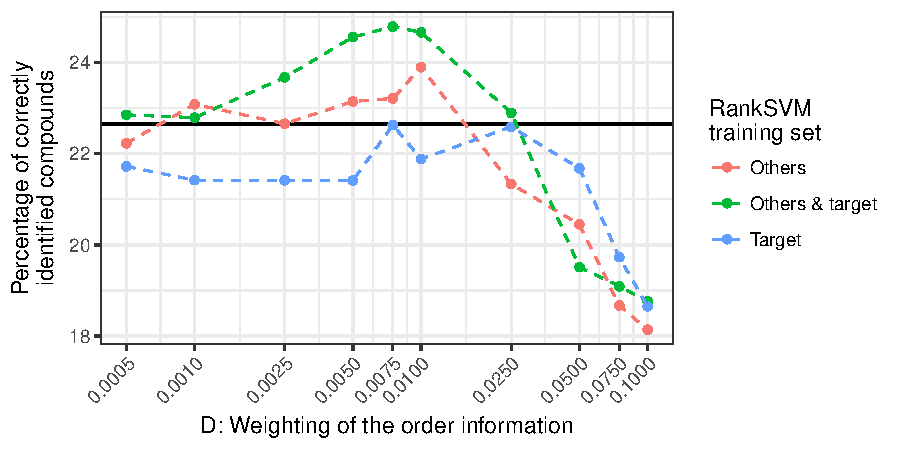
\includegraphics[width=\textwidth]{images/top1_accuracy_reranking_GS_BS_n_rep_1000_no_facet.pdf}
% \end{center}
% % \vspace{-0.25cm}
% \column{0.35\textwidth}
% \begin{block}{Observations}
% \begin{itemize}
%     \item Improved identification accuracy for \emph{Others} ($23.9\%$) and \emph{Others \& target} ($24.8\%$)
%     \item RankSVM trained only on the \emph{target} data cannot improve.
% \end{itemize}
% \end{block}
% \end{columns} 
    
\begin{figure}
    \centering
    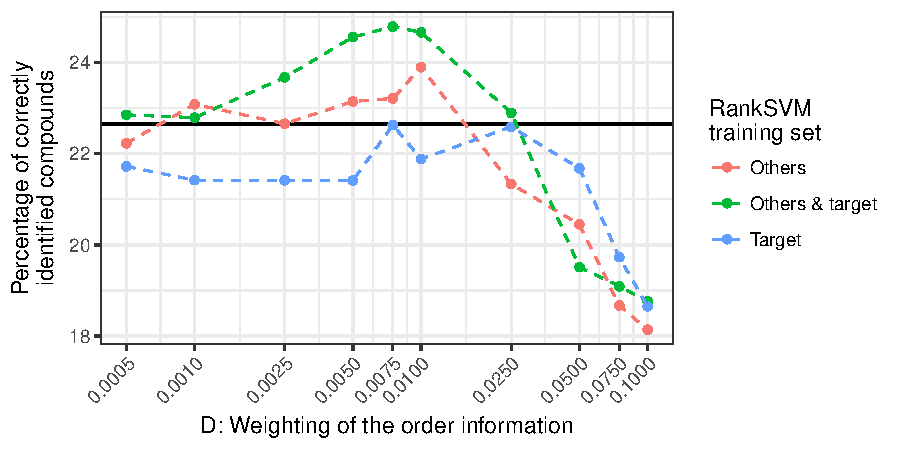
\includegraphics[width=0.9\textwidth]{images/top1_accuracy_reranking_GS_BS_n_rep_1000_no_facet.pdf}
\end{figure} 
\vspace{-0.35cm}
\begin{small}
% \only<1>{
% \begin{table}
%     \centering
% \begin{tabular}{l|c|c}
%     \toprule
%     (only) Target & $\Pref(\sys_{Impact})$ & 222 RTs\\
%     (only) Others & $\bigcup_{\sys \in \hat{S}} \Pref(s)$ & 1098 RTs\\
%     Others \& target & $\bigcup_{\sys \in \hat{S}} \Pref(s) \cup \Pref(\sys_{Impact})$ & 1320 RTs\\
%     \bottomrule
% \end{tabular}
% \end{table}
% }
\only<1>{
\begin{block}{Observations}
\vspace{-0.15cm}
\begin{itemize}
    \item Improved identification accuracy for \emph{Others} ($23.9\%$) and \emph{Others \& target} ($24.8\%$)
    \item RankSVM trained only on the \emph{target} data cannot improve.
\end{itemize}
\end{block}
}
\end{small}
}


% Summary frame
\section[$\Sigma$]{Summary}
\frame{
    \frametitle{Summary}  
    
% \begin{block}{Contribution}
\begin{small}
\begin{itemize}
    \item Proposed a method for predicting liquid chromatographic orders using RankSVM.
    \item Prediction model can be trained on retention time data from different chromatographic systems.
    \item Proposed method to integrate predicted retention orders and MS/MS scores for metabolite identification in LC-MS setting  
    \item Metabolite identification accuracy can be improved using predicted retention orders.
\end{itemize}
\end{small}
\vspace{-0.5cm}
\begin{footnotesize}
\begin{columns}[t]
\column{.49\textwidth}
\begin{block}{Acknowledgement}
This work has been supported by Academy of Finland and the Aalto Science-IT infrastructure. 
\\
Travel fellowship was granted from ECCB with support of the ISCB society.
\end{block}
\column{.49\textwidth}
\begin{alertblock}{Visit the poster at 18:30!}
ID: P\_Da080
\end{alertblock}
\begin{block}{Source code available}
\url{https://version.aalto.fi/gitlab/bache1/retention_order_prediction}
\end{block}
% \vspace{-0.15cm}
\end{columns}
\end{footnotesize}
}

\begin{appendix}

\printbibliography%[heading=none]d

\section{Liquid-Chromatography}

\frame[noframenumbering]{
    \frametitle{Liquid-Chromatography principle}
    
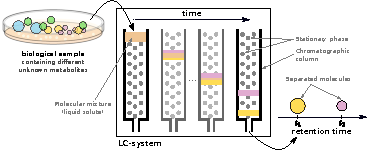
\includegraphics[width=\textwidth]{images/lc_concept.pdf}
}

\section{Molecular fingerprints}

\frame[noframenumbering]{
%     \frametitle{Compare binary and counting molecular fingerprints}
    \frametitle{Molecules represented using MACCS dictionary fingerprints}

\begin{figure}
    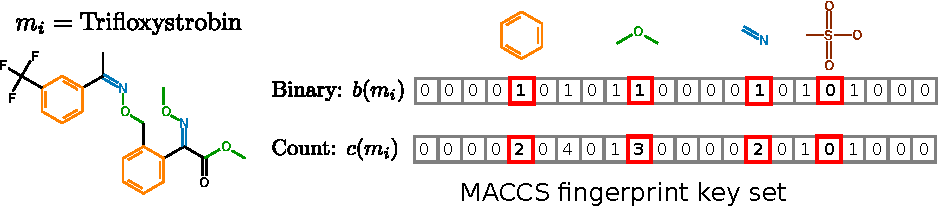
\includegraphics[width=\textwidth]{images/fingerprint_example.pdf}
\end{figure}
\begin{block}{Kernels used for the feature embedding in RankSVM}
\vspace{-0.25cm}
% \begin{small}
\begin{itemize}
    \item Binary: Tanimoto kernel \cite{Ralaivola2005}
\begin{center}
    $\kmol(m_i,m_j)=\frac{|b(m_i)\cap b(m_j)|}{|b(m_i)\cup b(m_j)|}$%\frac{b(m_i)^T b(m_j)}{b(m_i)^T b(m_i)+b(m_j)^T b(m_j)-b(m_i)^T b(m_j)}$
\end{center}
    \item Count: MinMax kernel \cite{Ralaivola2005}
\begin{center}
    $\kmol(m_i,m_j)=\frac{\sum_{s=1}^{N_{sub}}\min(c_s(m_i),c_s(m_j))}{\sum_{s=1}^{N_{sub}}\max(c_s(m_i),c_s(m_j))}$
\end{center}
\end{itemize}
% \end{small}
\end{block}
}

\frame[noframenumbering]{ 
    \frametitle{Compare binary and counting molecular fingerprints}
%     \framesubtitle{Encoding molecular structures using MACCS dictionary molecular fingerprints.}

\begin{itemize}
    \item Pairwise prediction accuracy ($\pm 2\sigma$) for different target systems
    \item RankSVM models trained using single system $\Pref(\sys)$.
\end{itemize}

\begin{table}[!t]
\begin{tabular}{@{}lcc@{}}
    \toprule 
    Target system $\sys$ & Binary MACCS & Counting MACCS \\\midrule
    Eawag\_XBridgeC18 & $0.796 (\pm 0.015)$ & $\mathbf{0.844 (\pm 0.011)}$ \\
    FEM\_long         & $0.882 (\pm 0.016)$ & $\mathbf{0.905 (\pm 0.015)}$ \\
    RIKEN             & $0.826 (\pm 0.024)$ & $\mathbf{0.848 (\pm 0.017)}$ \\
    UFZ\_Phenomenex   & $0.790 (\pm 0.027)$ & $\mathbf{0.802 (\pm 0.017)}$ \\
    LIFE\_old         & $0.842 (\pm 0.050)$ & $\mathbf{0.862 (\pm 0.035)}$ \\
    \bottomrule
\end{tabular}
\end{table} 
}


\end{appendix}

\end{document}
